\chapter{Evaluation} \label{chapter:evaluation}
This chapter is split into several sections, directly tied to the outcomes of the work achieved.
Firstly, we present the notes on the actual protocol specification, in light of examining and implementing a proof--of--concept on top of it.
We follow this up with a discussion of some of the testing aspects that were relevant to the proper analysis of the protocol and its implementation.
Furthermore, we give some more details on the choice of environment and tools (in essence, Mirage and some of the OCaml libraries) and the respective feedback on their usage.
Lastly, we provide a performance analysis of the system, with regards to storage efficiency, request latency and internal timings of cryptography operations.

\section{Nigori Protocol} \label{sec:evaluation:protocol}
As expected, working with a \wip protocol is a highly iterative task in the sense that there are many aspects that show themselves as potential areas of change.
One of the main such areas was overall protocol specificity.
Initially, while going through the RFC, in an attempt to understand the protocol and implement pieces of it, in a bottom--up approach, there were plenty of parts of the protocol's working that were either under or poorly specified.
The most explicit of them was the cryptography part.
Many of the primitives required by Nigori, and particularly the exact ways in which they were to be used or combined, was presented in a difficult to interpret format.
For example, the exact working of \myref{PBKDF} was left completety to its supporting RFC.
While this would seem natural for an RFC, the supporting document was not the easiest read to interpret and subsequently implement off of.
Yet another example was the description for the deterministic version of content encryption, \myref{EncDet}, which was slightly misleading, in the sense that internally, it uses an \myref{HMAC} (which outputs 20 bytes) and then shrinks that to the fixed size of an \myref{AES} initialization vector (16 bytes, in the current implementation), by splitting up the \myref{HMAC} into pieces of the required size and applying xor among them, which was not directly apparent from the specification.
Finally, the respective matching decryption primitives (as previously denoted by \myref{Dec} and \myref{DecDet}), are completely missing.
Nevertheless, most of these misunderstandings were resolved with direct communication with the RFC authors and access to the source code of the previous implementations, at specific points.

On a different note, in light of the implementation work, one aspect of the protocol became apparent and feedback and changes were brought to it to accommodate: the imposed strictness.
As it stands now, the protocol demands that all communication be done over HTTPS, with servers having valid certificates.
In our implementation, however, we have bypassed this requirement, in an attempt to make the server a proof--of--concept implementation.
The working of the protocol stays the same, nonetheless, just that the overall security of the data being transmitted now becomes susceptible to third party interceptions.
However, since no secret data is ever sent in plaintext, this should not be a serious concern.
Nevertheless, this does violate the \textbf{authentication} property of security protocols, as now the server does not have a valid means of proving its identity to the client.
However, we can argue that HTTPS certificates can also be faked, thus making this an attack vector that is peripheral to the protocol, per se.

Another area where the specification is rigid is with regards to which cryptography parts are being used.
For example, in our OCaml implementation, access to a proper, fully-working version of DSA, with support for key sized of up to the required 3072, was restricted.
As such, instead of mandating DSA, having some mechanism to negotiate the protocol to be used, for example, for the signing of the content, could have been useful.
Such a mechanism is already in place for determining the serialization formats that both client and server can and should use.
What is more, the Nigori specification also mandates the use of DSA with fixed internal parameters, that could be shared among the client and server libraries.
While this is done for obvious security reasons, as choosing these parameters affects the strength of the algorithm's working, this nevertheless leaves no options for platforms that do not have access to the mandated option.
Ultimately, this is a matter of choice and debate, between the flexibility offered by some form of algorithm negotiation phase and the potential security issues that can arise from using weak algorithms or weak parameters.
However, we believe that some form of middle-ground can be achieved, while also gauging and mandating a certain algorithmic strength of encryption.
At the very least, the system could mediate algorithms and key sizes and subsequently pass on to the client the parameters it should use, if the server is aware of sensible defaults for the options the client has available.

\section{Testing}
Short of using formal verification tools for the intricate pieces of the Nigori protocol, we resorted to pure functional testing.
As such, we took the respective library offered functionality as given and tested everything that was built on top of it accordingly.
Each of the cryptographic primitives was tested individually.
Furthermore, as per the client requirements, these primitives were also tested in combination and the results compared against running the same operations with external tools.

Also, the corresponding encryption and decryption steps were tested to work well combined.
Likewise, the respective JSON serialization and deserialization were also tested to perform as expected, when combined with the remainder of the system functionality (encoding / encryption).

Similarly, the server's database implementations for both the in--memory version and the SQLite backed one were tested in parallel, thanks to the module functorization capabilities of OCaml.
Thus, all of the provided functionality from the database was tested, under the various scenarios in which messages could be exchanged and commands could be subsequently issued, in light of those exchanges.
As such, proper test coverage was achieved on all code paths that were feasible, given the database interface provided.

This methodology of performing both individual unit tests for the simple pieces of protocol workings, together with integration testing for the modularly composed pieces was consistent with our generic approach to protocol design.
Furthermore, it proved fundamental when it came time to integrate the pieces into making the client and server interact.

\section{Mirage and OCaml Environment}
As initially expected and desired, the systems and toolchains we were working with were not fully production ready.
As such, many of them, on occasion, presented less than optimal behavior.
Overall, in light of our work, much feedback was brought to the various pieces in the Mirage and OCaml ecosystem which were used.
The most important parts are highlighted here.

As such, while the \myref{ocaml-cohttp} library provided very mature and stable support for the required HTTP functionality, less could be said about the respective SQLite implementation of the storage layer.

TODO: reiterate this:

Despite the ease that OCaml brought towards the modularity aspect of the implementation, there are still certain design differences between the actual in--memory storage version of the database and the physical storage one.
Moreover, there were also certain issues and quirks that took a certain amount of time to either identify and / or get around.
As such, we also include a discussion on these elements in what follows:
\begin{description}
  \item[Memory] the in--memory variant of the database makes use of the native library OCaml \myref{Hashtbl} datastructure.
  As expected, this is a hash table with parameterized keys and values.
  For this version of the database, we use an OCaml record to represent the internal \myref{type t}.
  This record keeps track of the \myref{User} related data (public keys and hashes), the actual data (\myref{indices}, \myref{revisions}, myref{data}) and finally, the metadata (\myref{nonces}).
  As previously mentioned, for security, we index the \myref{User} data, by the \myref{hash} and then the actual user data by instances of the \myref{User} module.
  Lastly, the only non--trivial or unexpected choice is related to the storing of nonces.
  While the \myref{Nonce} module allows for serializing instances to strings, OCaml does not provide a default \myref{Set} with O(1) access time.
  In absence of such, we store nonces, on a per user basis into yet another \myref{Hashtbl}, indexed from actual \myref{Nonce} instances to boolean values.

  \item[SQL] TODO: Quirks, problems and limitations.
\end{description}

Also, while arguably not directly related to Mirage, the respective library used for JSON serialization could have also used some improvements.
Primarily, the library offered the ability to annotate the ATDs with extra information that would be used in either the JSON form, or the OCaml form.
Some mechanism, such as pre and post serialization and deserialization hooks, could have helped a great deal with semi-automating the development process of the message formats.

TODO: some discussion about \myref{js\_of\_ocaml}.

\section{Performance}
For performance analysis, we decided we would primarily investigate three aspects of the system.
On the one hand, we would analyze the overall storage footprint and how this evolves with both number of items, as well as respective size of the individual items.
On the other hand, we realized it would also be important to have some analysis of the overall latency of performing requests -- such as \myref{/get} calls.

\subsection{Storage}
In order to properly test the overall behavior of the Nigori server and how much storage it consumes, we decided to analyze the persistent version of the server implementation, the one using SQLite.
We hypothesized that the database engine would naturally consume roughly as much space as we actually contributed to it.
As such, increasing the overall size of the data we insert into the database would lead to a matching increase in the overall amount of space taken by the database itself.
To test this appropriately, we filled the data store through a program that made direct calls to the database.
We varied both the total number of items to keep at any given time in the store, from 1 to 10000, by factors of ten, while also varying the size of the individual items being saved.
Since an item is defined by three components, an index, a revision and the actual data, we decided to fix two of these, the index and the revision, to some pre-determined size (32 bytes), as these should in a sense be metadata.
For the actual data, we initially experimented with small items, of the order of 100 bytes, to 1600 bytes, however, we noticed considerable bias at those sizes.
As such, we decided to choose larger values to understand what was happening.
We took five samples and varied the sizes by factors of two, starting from 4kb, to 64kb.
The results are presented in Figure \ref{fig:storage}.

\begin{figure}
\centering
\begin{subfigure}{.5\textwidth}
  \centering
  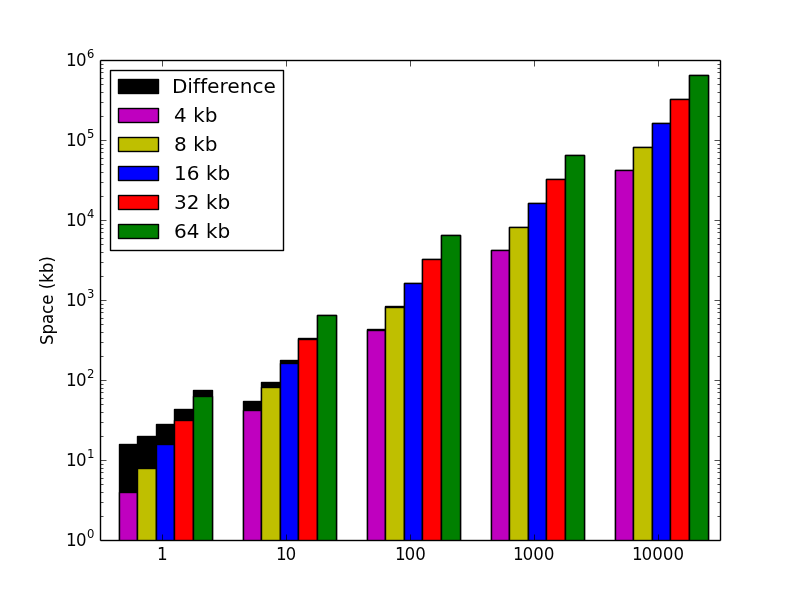
\includegraphics[width=1.1\linewidth]{images/storage_numbers}
  \caption{Clustering by number of items.}
\end{subfigure}%
\begin{subfigure}{.5\textwidth}
  \centering
  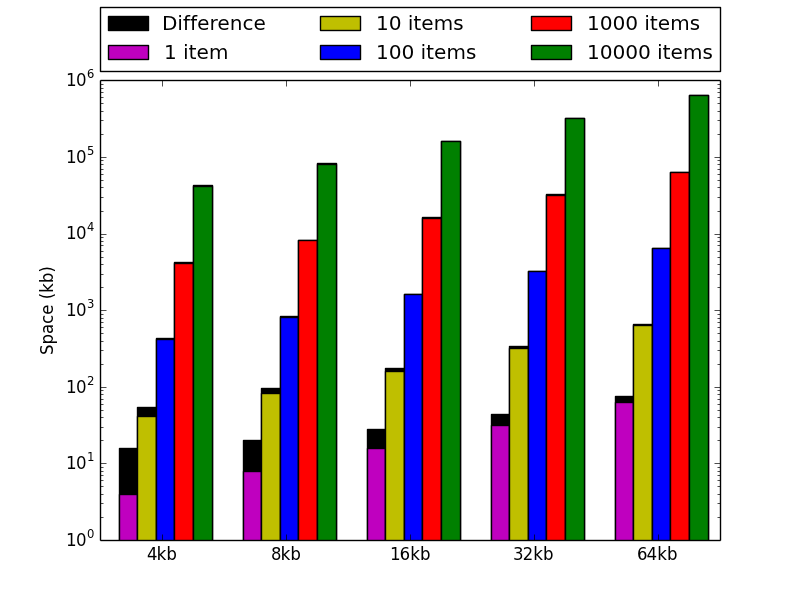
\includegraphics[width=1.1\linewidth]{images/storage_values}
  \caption{Clustering by size of data.}
\end{subfigure}
\caption{Variation of storage requirements with number of items and size of data.}
\label{fig:storage}
\end{figure}

% \myfig{Variation of storage requirements with number of items and size of data.}{storage}{0.8} \label{fig:storage}

The graphs are log--log scale, as we are expecting the storage to vary proportionally to our factorization, keeping one parameter fixed.
Thus, for example, doubling the size of the data while keeping the number of items fixed, we expected the storage requirements to double.
After some simple calculations of expected values, we realized there is some apparent inconsistency.
To that end, we also graphed the difference between our calculations and the actual data.
We present two graphs of the same data, clustered once by the number of items and once by size of data, two show the linear increase more clearly in both cases.

\begin{table}[H]
  \centering
  \begin{tabular}{|c| |*{5}{c|}}
  \hline
  \backslashbox{Items}{Size (kb)}  & 4 & 8 & 16 & 32 & 64 \\\hline
  1 & \myss{11}{73.17} & \myss{11}{58.54} &\myss{11}{41.81} & \myss{11}{26.61} & \myss{11}{15.40} \\\hline
  10 & \myss{13}{23.60} & \myss{13}{13.66} & \myss{14}{7.94} & \myss{15}{4.44} &\myss{15}{2.28} \\\hline
  100 & \myss{17}{4.06} & \myss{17}{2.12} & \myss{26}{1.63} & \myss{42}{1.31} & \myss{42}{0.66}\\\hline
  1000 & \myss{72}{1.70} &  \myss{72}{0.88} & \myss{157}{0.96} & \myss{324}{1.00} & \myss{324}{0.50}\\\hline
  10000 &\myss{619}{1.46} & \myss{619}{0.75} & \myss{1461}{0.89} & \myss{3142}{0.97} & \myss{3142}{0.49} \\\hline
  \end{tabular}
  \caption{Table of differences between experimental and expected storage data (raw and percentages).}
  \label{table:storage}
\end{table}

The raw difference (rounded to kbs) and the percentage it represents of the actual data is listed in Table \ref{table:storage}.
To compute the difference, we took into consideration the pieces we use in the encryption mechanism of both index, revisions and values.
As such, we have a 16 byte initialization vector, a 20 byte \myref{HMAC} hash and a cypher text generated by \myref{AES} which is always a multiple of 16 bytes (hence our selection of 32 byte index and revision).
This gives us an overhead of 68 bytes for our choice of index and revision.
As we were using the SQLite backend, we also needed to account for the issues that we had to bypass from the ORM.
As such, per data item, we also keep, for foreign key mechanics, both a \myref{SHA-1} hash of the user's public key (16 bytes) and a reference to the actual index of the data (thus 68 bytes).

Even with our predictions, we still see a considerable overhead at small numbers and data values, which we can attribute to the base requirements the ORM might have.
As we increase the number of items, we see that, percentage wise, the difference drops significantly, to below 1\% values.
We attribute those final inconcistencies again to ORM internals such as any database indexes and primary keying that might be happening in the background.

The most important result, however, is the linear increase presented on our log--log graphs.
This tells us that the database engine behaves as we expect and increasing either data size or number of items by a certain factor, triggers a similar increase in the overall storage, by the same factor.

\subsection{Latency}
This part of the analysis makes use of the data stores previously generated in the storage analysis, as those offer us content at various fill rates.
As such, the evaluation is split into several parts.
Initially, we were considering looking at both \myref{/put} and \myref{/get} operations, and how their latency response changes.
However, we decided to take a step back and look at the big picture and the individual pieces of a request, before we proceed.
Thus, every request can be split into three major time components: time spent explicitly on the client side (encryption and packaging of message), time spent on the medium of travel (in the internals of the HTTP library, in the kernel networking stack and in transmission) and finally time spent on the server (unpacking the request, executing against the database, packing the response).
This realization caused us to add modifications to the implementation, to be used for the latency evaluation part, by having both client and server report their respective times.
Subsequently, this subsection analyzes these three components, separately.

\paragraph{Server} ~\\
Our first experiments used the previous storage data to issue \myref{/get} commands and just analyze the timing data we obtained.
However, this made us realize that, for example, varying the number of items that the database contains does not affect the time spent on the medium, or on the client side, whatsoever.
As such, we decided to use all of this data and instead, show how the server performs with regards to these requests.
We decided to only execute \myref{/get} requests, instead of \myref{/put} requests, so as to not pollute the database content.
Moreover, we wanted to execute a certain number of requests for each individual instance of parameters (number of items, size of data) of the database and subsequently obtain the mean and standard deviation of the times.
Since we have collections with small numbers of items, we considered that issuing \myref{/put} requests would distrupt the results of our analysis, as the number of items would increase during tests.
Figure \ref{fig:time:server} shows the results of our analysis.

Bla.\label{fig:time:server}

\paragraph{Medium} ~\\
TODO:

\paragraph{Client} ~\\
TODO:

TODO: client side of timing; AES encryption at various rates and sizes of data; DSA signature of varying sizes

TODO: on the wire timing; discussion about HTTP layer in mirage libs; talk about kernel networking stack and respective stddev in data; explicit comments on variation with size of data; note on use of same machine and implicit time on wire being close to 0

TODO: server side of timing; DSA verification times?; database query times; discussion of means and increase with respect to both number of items and size of data
